In this section we propose a way to model a set of \ewhc{}, $\Lambda$, as an automaton, by utilising the satisfaction set $\sset{}{ \Lambda }$ and the concept of \emph{dominant set}.
The presented approach is invariant to the control system dynamics. 
For this reason, the resulting model can be used as an interface that separates the software design phase from the stability analysis (Section~\ref{sec:stability}), allowing the complete architecture analysis to be decoupled.

%\subsection{Constraint graph}%
%\label{sec:constraint_graph}
%%
%An \ewhc{}, as presented in Definition~\ref{def:new-mk}, can be systematically represented using an \emph{automaton} and the corresponding directed labeled graph.
%Each vertex in the graph corresponds to a subword of the last $k$ outcomes of the extended weakly-hard task executions. 
%Trivially, there exists no vertices for subwords that do not satisfy the \ewhc{}.
%A directed labeled edge connects two vertices if and only if the outcome $\event$ -- the edge's label -- appended to the tail vertex's subword representation would result in an equivalent one to the head vertex's.
%This implies that a random walk in the graph corresponds to a random word satisfying the \ewhc{}.
%Particularly, this implies that all the walks in the graph corresponds to \emph{all} words satisfying the \ewhc{}, i.e., $\sset{}{\lambda^{\strat}}$.
%
%\begin{figure}[t]
%    \begin{minipage}[c]{0.48\textwidth}
    \begin{center}
        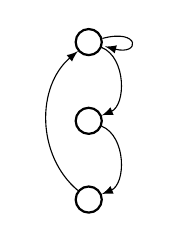
\begin{tikzpicture}[>=latex]
            \node[draw, thick, circle, radius=0.4] (a) at (0,0) {$\cX\cH\cH$};
            \node[draw, thick, circle, radius=0.4] (b) at (0,-1) {$\cH\cH\cM$};
            \node[draw, thick, circle, radius=0.4] (c) at (0,-2) {$\cH\cM\cH$};
            \draw[->] (a) edge [loop right] node[right] {$\cH$} (a);
            \draw[->] (a) edge [bend left=67.5] node[right] {$\cM$} (b);
            \draw[->] (b) edge [bend left=67.5] node[right] {$\cH$} (c);
            \draw[->] (c) edge [bend left=50] node[left] {$\cH$} (a);
        \end{tikzpicture}

        (Example~\ref{ex:auto-kill})\\[1pt]
        $\lambda^{\strat} = \overbar{\binom{1}{3}}^{\text{Kill}}$
    \end{center}
\end{minipage}
%
%    \begin{minipage}[c]{0.48\textwidth}
    \begin{center}
        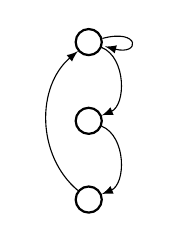
\begin{tikzpicture}[>=latex]
            \node[draw, thick, circle, radius=0.4] (a) at (0,0) {$\cX\cT\cH$};
            \node[draw, thick, circle, radius=0.4] (b) at (0,-1) {$\cT\cH\cM$};
            \node[draw, thick, circle, radius=0.4] (c) at (0,-2) {$\cH\cM\cR$};
            \draw[->] (a) edge [loop right] node[right] {$\cH$} (a);
            \draw[->] (a) edge [bend left=67.5] node[right] {$\cM$} (b);
            \draw[->] (b) edge [bend left=67.5] node[right] {$\cR$} (c);
            \draw[->] (c) edge [bend left=50] node[left] {$\cH$} (a);
        \end{tikzpicture}

        (Example~\ref{ex:auto-skip})\\[1pt]
        $\lambda^{\strat} = \overbar{\binom{1}{3}}^{\text{Skip-Next}}$
    \end{center}
\end{minipage}
%
%    \caption{Minimal graph $\GG{\lambda^{\strat}}^*$ for Examples 1 and 2.}
%    \label{fig:min-graph}
%\end{figure}
%
%We denote the graph corresponding to a task $\tau\vdash\lambda^{\strat}$ with the symbol $\GG{\lambda^{\strat}} = (\VV{\lambda^{\strat}}, \EE{\lambda^{\strat}})$.
%Here, $\VV{\lambda^{\strat}}$ represents the set of \emph{vertices} in the graph and $\EE{\lambda^{\strat}}$ represents the set of \emph{edges} (also denoted \emph{transitions}).
%Each vertex $v_i \in \VV{\lambda^{\strat}}$ corresponds to a word $\aword_i \in \sset{k}{\lambda^{\strat}}$.
%A \emph{subword} $\aword_i\left(a..b\right)$ of $\aword_i = \left\{ \event_1, \dots, \event_N \right\}$ is a new word containing the characters from position $a$ to position $b$, i.e., $\aword_i\left(a..b\right) = \left\{ \event_a, \dots, \event_b \right\}$.
%We use $\aword_i\left(a..\text{end}\right)$ to indicate the subword from position $a$ till the end of $\aword_i$.
%%
%A transition $e = (v_i,v_j,\event)\in \EE{\lambda^{\strat}}$, takes us from vertex $v_i$ to vertex $v_j$ and is labeled by the character $\event \in \Sigma\left(\strat\right)$.
%Vertex $v_j$ is said to be a direct successor of $v_i$ if concatenating the character $\event$ to the end of the vertex's word $\aword_i\left(2..end\right)$ gives $\aword_j$.
%
%Intuitively, a graph $\GG{\lambda^{\strat}}$ has \emph{at most} a number of vertices equal to the cardinality of the set of feasible words $\sset{k}{\lambda^{\strat}}$, or formally $\abs{\VV{\lambda^{\strat}}} \leq \abs{\sset{k}{\lambda^{\strat}}}$.
%However, to avoid unnecessary complexity, a \emph{minimal automaton} $\GG{\lambda^{\strat}}^*=(\VV{\lambda^{\strat}}^*, \EE{\lambda^{\strat}}^*)$ is easily obtained from $\GG{\lambda^{\strat}}$ using standard techniques~\cite{Hopcroft:2001}.
%Given two vertices $v_{i}$ and $v_{j}$, if they share the same successors with the same transition labels (i.e., outcomes) $\event$ they are considered equivalent and thereby combined.
%The differing characters in the word representations of $v_i$ and $v_j$ are replaced by an \emph{any outcome} token, which we denote with $\cX$.
%This process is repeated until the automaton can no longer be reduced.
%%
%When considering the Skip-Next strategy, an additional auxiliary token $\cT$ is introduced to represent all outcomes where a job is completed (ergo; $\cT = \left\{ \cH,\, \cR \right\}$).
%
%
%%\afterpage{%
%%    \clearpage
%    \begin{figure*}[h]
%        \begin{minipage}[c]{0.4\textwidth}
    \begin{center}
        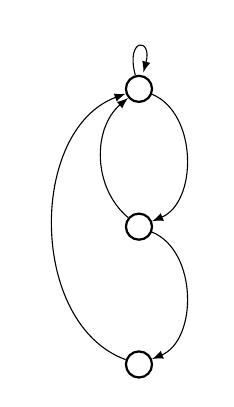
\begin{tikzpicture}[>=latex]
            \node[draw, thick, circle, radius=0.4] (a) at (0,0) {$\textcolor{white}{\cH}\cX\cX\cH\textcolor{white}{\cH}$};
            \node[draw, thick, circle, radius=0.4] (b) at (0,-1.75) {$\textcolor{white}{\cH}\cX\cH\cM\textcolor{white}{\cH}$};
            \node[draw, thick, circle, radius=0.4] (c) at (0,-3.5) {$\textcolor{white}{\cH}\cH\cM\cM\textcolor{white}{\cH}$};
            \draw[->] (a) edge [loop above] node[above] {$\cH$} (a);
            \draw[->] (a) edge [bend left=67.5] node[right] {$\cM$} (b);
            \draw[->] (b) edge [bend left=50] node[left] {$\cH$} (a);
            \draw[->] (b) edge [bend left=67.5] node[right] {$\cM$} (c);
            \draw[->] (c) edge [bend left=70] node[left] {$\cH$} (a);
        \end{tikzpicture}

        (Constraint 1)\\[1pt]
        $\lambda^{\strat}_1 = \overbar{\left<2\right>}^{\text{Kill}}$
    \end{center}
\end{minipage}
\hspace{1cm}
\begin{minipage}[c]{\textwidth}
    \begin{center}
        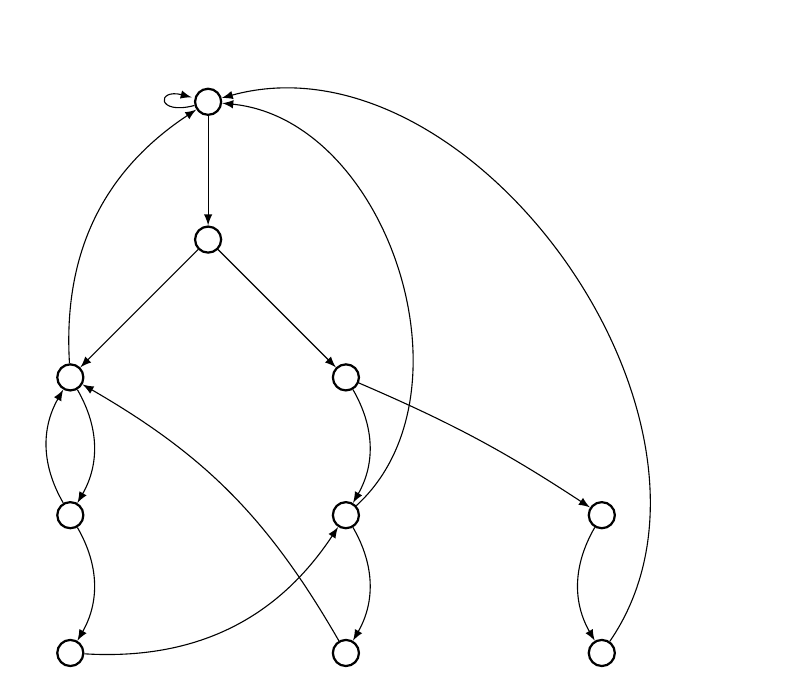
\begin{tikzpicture}[>=latex]
            \node[draw, thick, circle, radius=0.4] (a) at (0,0) {$\cX\cX\cX\cH\cH$};
            \node[draw, thick, circle, radius=0.4] (b) at (0,-1.75) {$\cX\cX\cH\cH\cM$};
            \node[draw, thick, circle, radius=0.4] (c) at (-1.75,-3.5) {$\cX\cX\cH\cM\cH$};
            \node[draw, thick, circle, radius=0.4] (d) at (-1.75,-5.25) {$\cX\cH\cM\cH\cM$};
            \node[draw, thick, circle, radius=0.4] (e) at (-1.75,-7) {$\cH\cM\cH\cM\cM$};
            \node[draw, thick, circle, radius=0.4] (f) at (1.75,-3.5) {$\cX\cH\cH\cM\cM$};
            \node[draw, thick, circle, radius=0.4] (g) at (1.75,-5.25) {$\cX\cH\cM\cM\cH$};
            \node[draw, thick, circle, radius=0.4] (h) at (1.75,-7) {$\cH\cM\cM\cH\cM$};
            \node[draw, thick, circle, radius=0.4] (i) at (5,-5.25) {$\cH\cH\cM\cM\cM$};
            \node[draw, thick, circle, radius=0.4] (j) at (5,-7) {$\cH\cM\cM\cM\cH$};

            \draw[->] (a) edge [loop left] node[left] {$\cH$} (a);
            \draw[->] (a) edge [] node[right] {$\cM$} (b);
            \draw[->] (b) edge node [above] {$\cH$} (c);
            \draw[->] (b) edge node [above] {$\cM$} (f);
            \draw[->] (c) edge [bend left] node [left] {$\cH$} (a);
            \draw[->] (c) edge [bend left] node [right] {$\cM$} (d);
            \draw[->] (d) edge [bend left] node [left] {$\cH$} (c);
            \draw[->] (d) edge [bend left] node [right] {$\cM$} (e);
            \draw[->] (e) edge [bend right] node [below] {$\cH$} (g);
            \draw[->] (f) edge [bend left] node [right] {$\cH$} (g);
            \draw[->] (f) edge [bend left=5] node [above] {$\cM$} (i);
            \draw[->] (g) edge [bend right = 66] node [right] {$\cH$} (a);
            \draw[->] (g) edge [bend left] node [right] {$\cM$} (h);
            \draw[->] (h) edge [bend right = 15] node [above] {$\cH$} (c);
            \draw[->] (i) edge [bend right] node [left] {$\cH$} (j);
            \draw[->] (j) edge [bend right = 70] node [right] {$\cH$} (a);

        \end{tikzpicture}

        (Constraint 2)\\[1pt]
        $\lambda^{\strat}_2 = \overbar{\binom{3}{5}}^{\text{Kill}}$
    \end{center}
\end{minipage}
\hspace{1cm}
\begin{minipage}[c]{0.8\textwidth}
    \begin{center}
        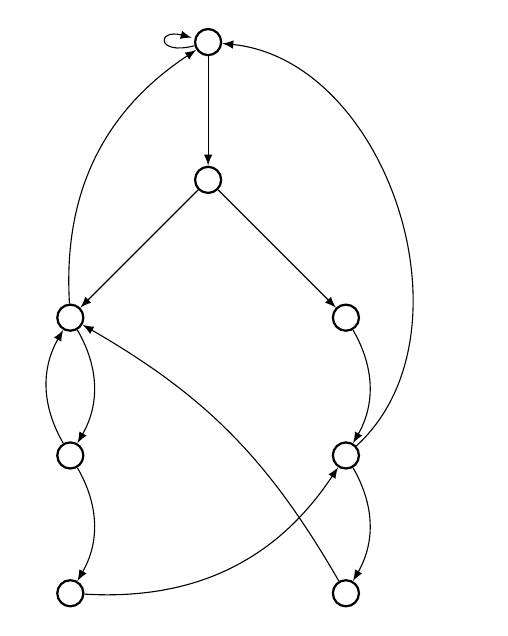
\begin{tikzpicture}[>=latex]
            \node[draw, thick, circle, radius=0.4] (a) at (0,0) {$\cX\cX\cX\cH\cH$};
            \node[draw, thick, circle, radius=0.4] (b) at (0,-1.75) {$\cX\cX\cH\cH\cM$};
            \node[draw, thick, circle, radius=0.4] (c) at (-1.75,-3.5) {$\cX\cX\cH\cM\cH$};
            \node[draw, thick, circle, radius=0.4] (d) at (-1.75,-5.25) {$\cX\cH\cM\cH\cM$};
            \node[draw, thick, circle, radius=0.4] (e) at (-1.75,-7) {$\cH\cM\cH\cM\cM$};
            \node[draw, thick, circle, radius=0.4] (f) at (1.75,-3.5) {$\cX\cH\cH\cM\cM$};
            \node[draw, thick, circle, radius=0.4] (g) at (1.75,-5.25) {$\cX\cH\cM\cM\cH$};
            \node[draw, thick, circle, radius=0.4] (h) at (1.75,-7) {$\cH\cM\cM\cH\cM$};

            \draw[->] (a) edge [loop left] node[left] {$\cH$} (a);
            \draw[->] (a) edge [] node[right] {$\cM$} (b);
            \draw[->] (b) edge node [above] {$\cH$} (c);
            \draw[->] (b) edge node [above] {$\cM$} (f);
            \draw[->] (c) edge [bend left] node [left] {$\cH$} (a);
            \draw[->] (c) edge [bend left] node [right] {$\cM$} (d);
            \draw[->] (d) edge [bend left] node [left] {$\cH$} (c);
            \draw[->] (d) edge [bend left] node [right] {$\cM$} (e);
            \draw[->] (e) edge [bend right] node [below] {$\cH$} (g);
            \draw[->] (f) edge [bend left] node [right] {$\cH$} (g);
            \draw[->] (g) edge [bend right = 66] node [right] {$\cH$} (a);
            \draw[->] (g) edge [bend left] node [right] {$\cM$} (h);
            \draw[->] (h) edge [bend right = 15] node [above] {$\cH$} (c);

        \end{tikzpicture}

        (Result)\\[1pt]
        $\Lambda^{\strat}_0 = \left\{ \lambda^{\strat}_1,\, \lambda^{\strat}_2 \right\}$
    \end{center}
\end{minipage}

%        \caption{Minimal graphs $\GG{\lambda^{\strat}_1}^*$, $\GG{\lambda^{\strat}_2}^*$, and $\GG{\Lambda^{\strat}_0}^*$ for Example~\ref{ex:auto-comb}.}
%        \label{fig:multi-graphs}
%    \end{figure*}
%%    \clearpage
%%}
%
%\begin{example}%
%    \label{ex:auto-kill}%
%    \emph{Given an \ewhc{},} $\lambda^{\strat} = \overbar{\binom{1}{3}}^{\text{Kill}}$\emph{, the minimal realisation $\GG{\lambda^{\strat}}^*$ is shown in the left-hand side of Figure~\ref{fig:min-graph}.
%    The vertex represented by the word $\cX\cH\cH$ is obtained by merging $\cH\cH\cH$ and $\cM\cH\cH$.}
%\end{example}
%
%\begin{example}%
%    \label{ex:auto-skip}%
%    \emph{Given an \ewhc{},} $\lambda^{\strat} = \overbar{\binom{1}{3}}^{\text{Skip-Next}}$\emph{, the minimal realisation $\GG{\lambda^{\strat}}^*$ is shown in the right-hand side of Figure~\ref{fig:min-graph}.}
%\end{example}
%
%The minimal automaton for Kill and Skip-Next in Figure~\ref{fig:min-graph} have identical number of vertices but slightly different transitions.
%This is not a coincidence, but follows directly from Definition~\ref{def:new-mk} and the extended alphabet $\Sigma\left(\strat\right)$.
%A hit ($\cH$) and a recovery ($\cR$) are both considered job completions, which is why the graphs for the Kill and Skip-Next strategies have the same structure.
%It is only the first job completion after a period of no job completions ($\cM$) that differ.
%However, the different transitions of the two graphs affect the corresponding closed-loop systems, as will be clear in Section~\ref{sec:stability}.
%
%\subsection{Dealing with multiple constraints}
%\label{sec:mult-const}
%
%The approach presented above for constructing a minimal automaton can be extended to the case where the task $\tau$ is subject to a set of multiple \ewhc{}. 
%Such a set is formally denoted as $\Lambda^{\strat}$.
%%
%In order to optimise the problem of building the minimal automaton of the corresponding system, it is beneficial that the set $\Lambda^{\strat}$ contains only constraints that cannot be further reduced using the hardness relations of Definition~\ref{def:domination}. 
%To this end, we first introduce the new concept of \emph{dominant (constraint) set}.
%%
%\begin{definition}[Dominant set]%
%    \label{def:dominant-set}%
%    %
%    Given a set of \ewhc{}, $\Lambda^{\strat}$, the set $\Lambda^{\strat}_0 \subseteq \Lambda^{\strat}$ is called the \emph{dominant set} of $\Lambda^{\strat}$ if:
%    \begin{enumerate}[label=(\roman*)]
%        \item $\lambda^{\strat}_i,\lambda^{\strat}_j \in \Lambda^{\strat}_0 \,\,\implies \lambda^{\strat}_i \npreceq \lambda^{\strat}_j,\, \forall i \neq j,$
%        \item $\lambda^{\strat}_i \in \Lambda^{\strat} \setminus \Lambda^{\strat}_0 \implies
%            \lambda^{\strat}_j \preceq \lambda^{\strat}_i,\, \exists \lambda^{\strat}_j \in \Lambda^{\strat}_0.$
%    \end{enumerate}
%\end{definition}
%
%Building upon Definition~\ref{def:satisfaction}, the satisfaction set of $\Lambda^{\strat}_0$ can be derived as follows, for $N\geq 1$:
%%
%\begin{equation}
%    \label{eq:satisfaction-multi}
%    \sset{N}{\Lambda^{\strat}_0} \equiv \bigcap_{\lambda^{\strat}_i \in \Lambda^{\strat}_0} \sset{N}{\lambda^{\strat}_i}.
%\end{equation}
%%
%We can then obtain a minimal graph $\GG{\Lambda^{\strat}_0}^*$ following a procedure similar to the one presented for a single constraint $\lambda^{\strat}$ in Section~\ref{sec:state-machine}.
%As a first step, the length of the words in each vertex of the corresponding graph must be defined.
%Since $\Lambda^{\strat}_0$ may contain constraints with different window values, the choice is not straightforward.
%We propose a safe assumption about the word length $k_0$, defined as $\,k_0 = \max_{k} \lambda^{\strat},\,\, \forall \lambda^{\strat} \in \Lambda^{\strat}_0$.
%An algorithm can then be built that adds vertices, with word representations $\aword_i \in \sset{k_0}{ \Lambda^{\strat}_0 }$, to the graph until a minimal realisation is generated.
%The obtained graph is finally passed through a post-processing step (strategy-dependent) that assigns the appropriate transitions in order to obtain a correct minimal automaton realisation $\GG{\Lambda^{\strat}_0}^*$.
%
%\begin{example}%
%    \label{ex:auto-comb}%
%    \emph{Given two \ewhc{},} $\lambda^{\strat}_1 = \overbar{\left<2\right>}^{\text{Kill}}$\emph{ and } $\lambda^{\strat}_2 = \overbar{\binom{3}{5}}^{\text{Kill}}$\emph{, the minimal realisation graphs $\GG{\lambda^{\strat}_1}^*$ and $\GG{\lambda^{\strat}_2}^*$ are shown as the leftmost and middle graphs of Figure~\ref{fig:multi-graphs}.
%    Generating the graph $\GG{\Lambda^{\strat}_0}^*$ from the dominant set $\Lambda^{\strat}_0 = \{ \lambda^{\strat}_1, \lambda^{\strat}_2 \}$ results in the rightmost graph of Figure~\ref{fig:multi-graphs}, satisfying both $\lambda^{\strat}_1$ and $\lambda^{\strat}_2$.}
%\end{example}
%
%
%Building a minimal automaton by choosing the dominant set $\Lambda^{\strat}_0$ improves the computational performance of the analysis.
%Nonetheless, the analysis presented in the following sections can be applied to any graph built from a given set $\Lambda^{\strat}$.
%To limit complexity in the notation, and for the sake of generality, all future steps will consider a generic graph $\GG{\Lambda^{\strat}}=(\VV{\Lambda^{\strat}}, \EE{\Lambda^{\strat}})$.
%
%
%\subsection{Dynamic model of a graph}
%\label{ssec:dynamicgraph}
%
%Extracting all the transitions in $\EE{\Lambda^\strat}$ corresponding to a character $\event$ yields what is generally known as a \emph{directed adjacency matrix}~\cite{xu2012matrix}, denoted here as a \emph{transition matrix}.
%\begin{definition}[Transition matrix]
%    \label{def:transition}
%    Given a graph $\GG{\Lambda^\strat}$, the \emph{transition matrix} $F_{\event} ( \GG{\Lambda^\strat} ) \in \R^{\abs{\VV{\Lambda^\strat}} \times \abs{\VV{\Lambda^\strat}}}$ with $\event\in\Sigma\left(\strat\right)$, is computed as $F_{\event} ( \GG{\Lambda^\strat} ) = \{f_{i,j}(\event)\}$ with
%    %
%    \begin{equation*}
%        f_{i,j}\funof{\event}=
%        \begin{cases}
%            1, &\text{ if } \exists \, e=(v_j,v_i,\event) \in \EE{\Lambda^\strat} \\
%            0, &\text{ otherwise.}
%        \end{cases}
%        \end{equation*}%
%\end{definition}
%%
%Since there can only exist \emph{at most one} successor from each vertex with a transition labeled with $\event$, the transition matrix $F_\event$ will thus have a column sum of either 1 or 0.
%We introduce a vector $q_t\in \R^{\abs{\VV{\Lambda^\strat}}}$ called \emph{G-state} (for graph state), representing the state of the given graph $\GG{\Lambda^\strat}$, which is associated to the interval $\pi_t$.
%This vector is formally defined as follows.
%\begin{definition}[G-state $q_t$]\label{def:qt}
%    Given a graph $\GG{\Lambda^\strat} = (\VV{\Lambda^\strat}, \EE{\Lambda^\strat})$ and a sequence $\aword \in \Sigma\left( \strat \right)^N$, for $k = \abs{v},\,\, v\in\VV{\Lambda^\strat}$, we define $q_t\in \R^{\abs{\VV{\Lambda}}}$, where the $i$-th element $q_{t,i}$ is defined as:
%    \begin{equation*}
%        q_{t,i}=
%        \begin{cases}
%            1, &\text{ if } \aword\left(t-k..t-1\right) \equiv v_i \in \VV{\Lambda^\strat} \\
%            0, &\text{otherwise}.
%        \end{cases}
%    \end{equation*}
%\end{definition}
%In other words, the G-state $q_t$ is the vector representation of the vertex we are \emph{leaving} at step $t$.
%In this definition, $q_t=0$ means that the transition at step $t-1$ was infeasible for the graph.
%The G-state dynamics, given an arbitrary sequence $\aword=\{\alpha_1,\dots,\alpha_t,\dots,\}$, is then defined as $q_{t+1} = F_{\event} ( \GG{\Lambda^\strat} )\cdot q_t$.
%Hence, the following property from~\cite{xu2012matrix} holds.
%\begin{lemma}[Infeasible sequence]
%    \label{cor:Fseqnotinlambda}
%    If $\aword \notin \sset{N}{ \Lambda^\strat }$, then $F_{\aword} ( \GG{\Lambda^\strat} ) =
%    F_{\event_N} ( \GG{\Lambda^\strat} )\cdots F_{\event_2} ( \GG{\Lambda^\strat} )\cdot F_{\event_1} ( \GG{\Lambda^\strat} ) = 0$
%\end{lemma}
%Thus, if $q_t=0$ for any $t$, then $q_{t'}=0$ for $t' \geq t$.
